%%%%%%%%%%%%%%%%%%%%%%%%%%%%%%%%%%%%%%%%%
% Beamer Presentation
% LaTeX Template
% Version 1.0 (10/11/12)
%
% This template has been downloaded from:
% http://www.LaTeXTemplates.com
%
% License:
% CC BY-NC-SA 3.0 (http://creativecommons.org/licenses/by-nc-sa/3.0/)
%
%%%%%%%%%%%%%%%%%%%%%%%%%%%%%%%%%%%%%%%%%

%----------------------------------------------------------------------------------------
%	PACKAGES AND THEMES
%----------------------------------------------------------------------------------------

\documentclass{beamer}

\mode<presentation> {
	\usetheme{Madrid}
	
	%\setbeamertemplate{footline} % To remove the footer line in all slides uncomment this line
	%\setbeamertemplate{footline}[page number] % To replace the footer line in all slides with a simple slide count uncomment this line
	\setbeamertemplate{navigation symbols}{} % To remove the navigation symbols from the bottom of all slides uncomment this line
}

\usepackage{graphicx} % Allows including images
\usepackage{booktabs} % Allows the use of \toprule, \midrule and \bottomrule in tables
\usepackage{tikz}

\usepackage[]{biblatex}
\usepackage[utf8]{inputenc}
 
%----------------------------------------------------------------------------------------
%	TITLE PAGE
%----------------------------------------------------------------------------------------

\title[Einführung Git / GitHub ]{Einführung Git / GitHub} % The short title appears at the bottom of every slide, the full title is only on the title page

\author{Philippe Käufer}
\institute[HACK TO THE FUTURE] % Your institution as it will appear on the bottom of every slide, may be shorthand to save space
{
\textit{BY Philippe Käufer (Lizenz: CC BY-NC-SA 3.0)} \\
HACK TO THE FUTURE \\ % Your institution for the title page
\medskip
}
\date{\today} % Date, can be changed to a custom date


\begin{document}

\begin{frame}
\titlepage % Print the title page as the first slide
\end{frame}

\begin{frame}
\frametitle{Übersicht} % Table of contents slide, comment this block out to remove it
\tableofcontents % Throughout your presentation, if you choose to use \section{} and \subsection{} commands, these will automatically be printed on this slide as an overview of your presentation
\end{frame}

%----------------------------------------------------------------------------------------
%	PRESENTATION SLIDES
%----------------------------------------------------------------------------------------

%------------------------------------------------
\section{Motivation}
%------------------------------------------------

%------------------------------------------------
\begin{frame}[fragile]
\frametitle{Problemstellung}
\begin{columns}
    \column[T]{.50\textwidth}
    \textbf{Versionierung}\smallskip
    \begin{itemize}
    \item index.html
    \pause \item index-test.html
    \pause \item index-test2.html 
    \end{itemize}

    \column[T]{.50\textwidth} 
    \pause \textbf{Entwickeln im Team}\bigskip
    \\index.html
    
	\fontsize{8pt}{1.2}\selectfont
    \begin{verbatim}
+---------+           +---------+
|         |           |         |
|         | USB-Stick |         |
|         |  ------>  |         |
|   Ich   |           |   Du    |
|         |  Netzwerk |         |
|         |  ------>  |         |
|         |           |         |
+---------+           +---------+
    \end{verbatim}

  \end{columns}
\end{frame}
%------------------------------------------------


%------------------------------------------------
\section{Versionsverwaltung mit Git / Github}
%------------------------------------------------

%------------------------------------------------
\begin{frame}
\frametitle{Was ist Git / Github ?}

	\begin{itemize}
    \item Als Team gemeinsam an Projekten/Code arbeiten
    \item Plattform um quelloffene (OpenSource) Projekte mit der Welt zu teilen
    \end{itemize}

\begin{tikzpicture}[remember picture,overlay]  
  \node [xshift=-3.1cm,yshift=1.5cm] at (current page.south east)
    {
\includegraphics[width=1.5cm,height=1.5cm]{images/Git-Icon-1788C.png}};
    
  \node [xshift=-1cm,yshift=1.5cm] at (current page.south east)
      {
\includegraphics[width=1.5cm,height=1.5cm]{images/Octocat.jpg}};
\end{tikzpicture}

\end{frame}
%------------------------------------------------


%------------------------------------------------
\begin{frame}
\frametitle{Workflow}
\begin{figure}

\begin{figure}
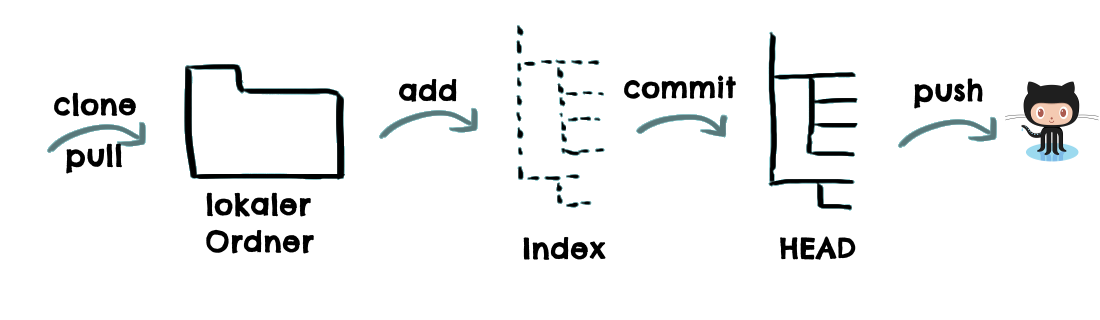
\includegraphics[scale=0.3]{images/trees.png}
\end{figure}

\end{figure}

\end{frame}
%------------------------------------------------


%------------------------------------------------
\section{Hands on}
%------------------------------------------------

%------------------------------------------------
\begin{frame}
\frametitle{Hands on}
\begin{figure}

\begin{itemize}
	\item Wie installiere ich Git (\url{https://git-scm.com/})
	\item Github und die Bedeutung bei httf
	\item Wie nutze ich Git (IDE / Tortoise)
\end{itemize}

\end{figure}
\end{frame}
%------------------------------------------------

%------------------------------------------------
\section{Cheat Sheet \& Linksammlung}
%------------------------------------------------

%------------------------------------------------
\begin{frame}
\frametitle{Cheat Sheet (Danke an Jugend Hackt)}
\begin{figure}

\includegraphics[scale=0.3]{images/Cheatsheet_git.png}
\end{figure}
\end{frame}
%------------------------------------------------

%------------------------------------------------
\begin{frame}
\frametitle{Linksammlung}
\url{\\\\wolf.shack} (Git + Tortoise)
\url{http://github.com}
\end{frame}
%------------------------------------------------

%------------------------------------------------
\begin{frame}
\frametitle{Quellen}

\begin{itemize}
    \item[] \url{https://rogerdudler.github.io/git-guide/index.de.html}
    \item[] \url{http://think-like-a-git.net/}
    \item[] \url{http://metaodi.ch/posts/2016/11/git-github-lightning-talk/}
\end{itemize}


\end{frame}
%------------------------------------------------

\end{document} 